\chapter{FreeRTOS kernel}
\label{freertos_kernel}

\section{Introduction}

FreeRTOS is a real-time operating system kernel (RTOS) for embedded devices. It has been ported to 35 microcontroller pletforms and has MIT open source licence hence the free in the name. \citep{freertos_licence}

Operating system (OS) is designed to be small and simple. The kernel itself has only three C files. It is written mostly in C with some assembly code included for scheduler routines.

FreeRTOS is ideally suited to deeply embedded real-time applications that use
microcontrollers or small microprocessors. This type of application normally includes a mix of
both hard and soft real-time requirements. \citep{freertos_mastering}

Soft real-time requirements are those that state a time deadline—but breaching the deadline
would not render the system useless. For example, responding to keystrokes too slowly might
make a system seem annoyingly unresponsive without actually making it unusable. \citep{freertos_mastering}

Hard real-time requirements are those that state a time deadline—and breaching the deadline
would result in absolute failure of the system. For example, a driver’s airbag has the potential
to do more harm than good if it responded to crash sensor inputs too slowly. \citep{freertos_mastering}

\noindent FreeRTOS features:

\begin{itemize}
    
    \item Pre-emptive or co-operative operation
    \item Very flexible task priority assignment
    \item Flexible, fast and light weight task notification mechanism
    \item Queues
    \item Binary and counting semaphores
    \item Mutexes
    \item Recursive mutexes
    \item Software timers
    \item Event groups
    \item Tick hook functions
    \item Idle hook functions
    \item Stack overflow checking
    \item Trace recording
    \item Task run-time statistics gathering
    \item Optional comemercial licensing and support
    \item Full interrupt nesting model (on some architectures)
    \item Tick-less capability for extreme low power applications
    \item Software manages interrrupt stack when appropriate (could save RAM space)
    
\end{itemize}

\noindent FreeRTOS file structure is shown in \autoref{fig:freertos_structure}.

\begin{figure}[H]
\dirtree{%
.1 Source.
.2 include.
.3 FreeRTOS.h.
.3 list.h - Primary structure used inside the kernel.
.3 message\textunderscore buffer.h.
.3 portable.h.
.3 projdefs.h.
.3 queue.h.
.3 semphr.h - Semaphores.
.3 stream\textunderscore buffer.h.
.3 task.h.
.3 timers.h - Software timers. 
.2 portable.
.3 [compiler] e.g{. GCC}.
.4 [architecture] e.g{. ARM\textunderscore CM4F}.
.5 port.c - Architecture and compiler specific.
.5 portmacro.c.
.3 MemMang.
.4 heap\textunderscore X.c - X is a heap number used.
.2 croutine.c.
.2 event\textunderscore groups.c.
.2 list.c.
.2 queue.c.
.2 stream\textunderscore buffer.c.
.2 tasks.c - Tasks and scheduler implementation.
.2 timers.c.
}
\caption{FreeRTOS file structure}
\label{fig:freertos_structure}
\end{figure}

\section{Inner workings of the tasks}
 

Every FreeRTOS task has a stack and a task control block, or short TCB. Kernel uses the TCB to manage tasks. A TCB contains all information necessary to completely describe the state of a task. \citep{freertos_inner_workings} A FreeRTOS task can exist in five states: running, blocked, ready, suspended and deleted. A state diagram is shown in \autoref{fig:freertos_task_states}.

\begin{figure}[H]

      \centering
      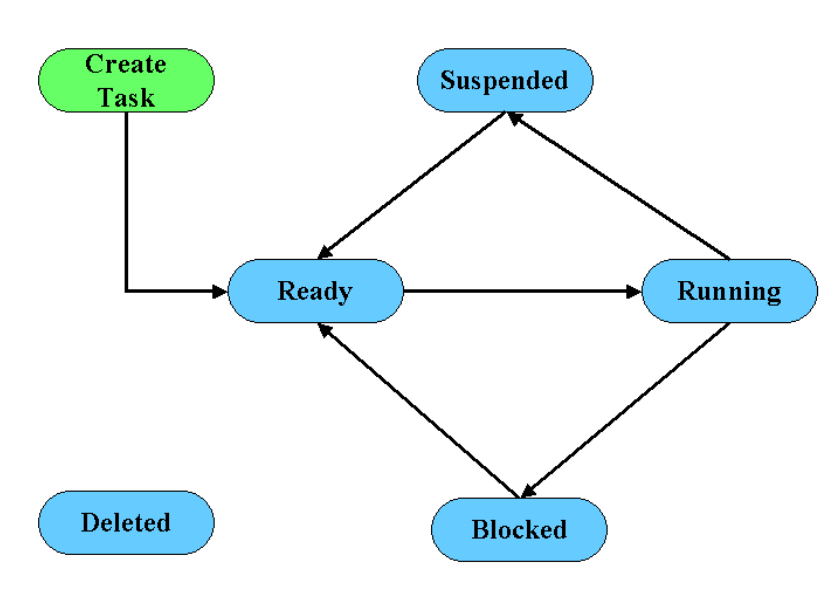
\includegraphics[width=0.7\linewidth]{images/freertos_task_states.png}
      \caption{FreeRTOS task states\citep[p~10]{freertos_inner_workings}}
      \label{fig:freertos_task_states}
    
\end{figure}

When a new task is created its TCB is populated. New tasks are immediately placed in a ready list. Whole scheduling is comprised of a lot of lists.

Ready list is arranged in order of priority with tasks of equal priority being serviced round robin. Ready list is not actually  a signle list, rather a configMAX\textunderscore PRIORITIES number of lists. Each priority level has a list for it. When scheduler looks for the next task it walks from the tasks with highest priority to the one with the lowest. Variable pxCurrentTCB points to a process in the ready list that is currently running.

The tasks in FreeRTOS can be blocked when accessing a resource that is not currently available. The scheduler blocks the tasks when they attempt to read from an empty container or write into a full one. This is also true for the semaphores, as they are a queue of size one in the background.

As indicated earlier, access attempts against queues can be blocking or non-blocking.
The distinction is made via the xTicksToWait variable which is passed into the queue
access request as an argument. If xTicksToWait is 0, and the queue is empty/full, the
task does not block. Otherwise, the task will block for a period of xTicksToWait
scheduler ticks or until an event on the queue frees up the resource.

Tasks can also be blocked without a use of containers. FreeRTOS provied vTaskDelay and vTaskDelayUntil functions for this purpose. When a task is delayed it is put onto a delay list. On every tick, scheduler checks if one of the tasks from the delay lists are unblocked. If they are, they are moved to the ready list.

Any task or, in fact, all tasks except the one currently running (and those servicing ISRs)
can be placed in the Suspended state indefinitely. Tasks that are placed in this state are
not waiting on events and do not consume any resource or kernel attention until they are
moved out of the Suspended state. When unsuspended, they are returned to the Ready state.

Finally, tasks can also be deleted. When delete is requested task is put in a deleted state. Deleted state is required because tasks are not deleted immediately after the call. Rather tasks are deleted, and its resources released, from the IDLE task. IDLE task has the lowest possible priority so this job may take some time.

\section{Inner workings of the scheduler}

This section gives a brief overview of a FreeRTOS scheduler.

\autoref{fig:freertos_scheduler_overview} shows an overview of the scheduler algorithm. The scheduler operates as a timer interrupt service routine that is called once every tick. Tick period is defined by configTICK\textunderscore RATE\textunderscore HZ. 

\begin{figure}[H]

      \centering
      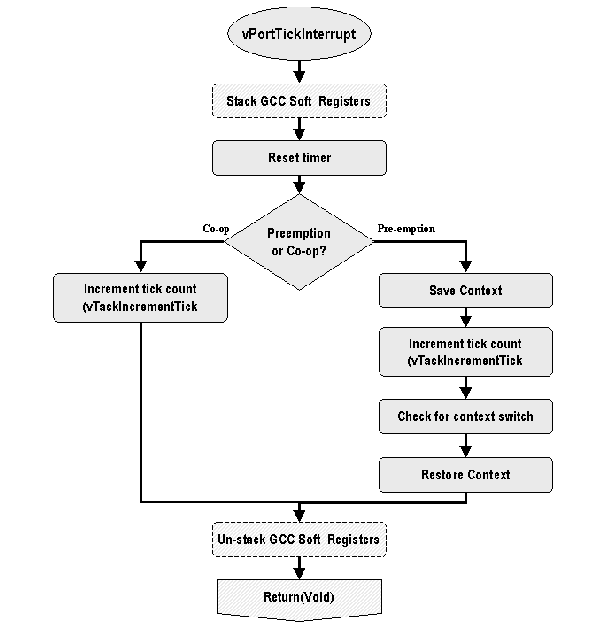
\includegraphics[width=0.8\linewidth]{images/freertos_scheduler_overview.png}
      \caption{Scheduler algorithm\citep[p~23]{freertos_inner_workings}}
      \label{fig:freertos_scheduler_overview}
    
\end{figure}

Context saving is done for the current task. Needed registers are saved on top of the task's stack. It is worth noting, when a task is first created its task is artificially filled. After saving the context scheduler increments the tick and checks if any other task with higher priority has been unblocked, or there is a task with same priority ready. Finally, context is restored and scheduler returns from the interrupt.  

\autoref{fig:freertos_scheduler_increment} shows the algorithm for vTaskIncrementTisk. vTaskIncrementTick is called once each clock tick by the HAL (whenever the timer ISR occurs). The right hand
branch of the algorithm deals with normal scheduler operation while the left hand branch
executes when the scheduler is suspended. As discussed earlier, the right hand branch
simply increments the tick count and then checks to see if the clock has overflowed. If
that’s the case, then the DelayedTask and OverflowDelayedTask list pointers are
swapped and a global counter tracking the number of overflows is incremented. An
increase in the tick count may have caused a delayed task to wake so check is performed.

\begin{figure}[H]

      \centering
      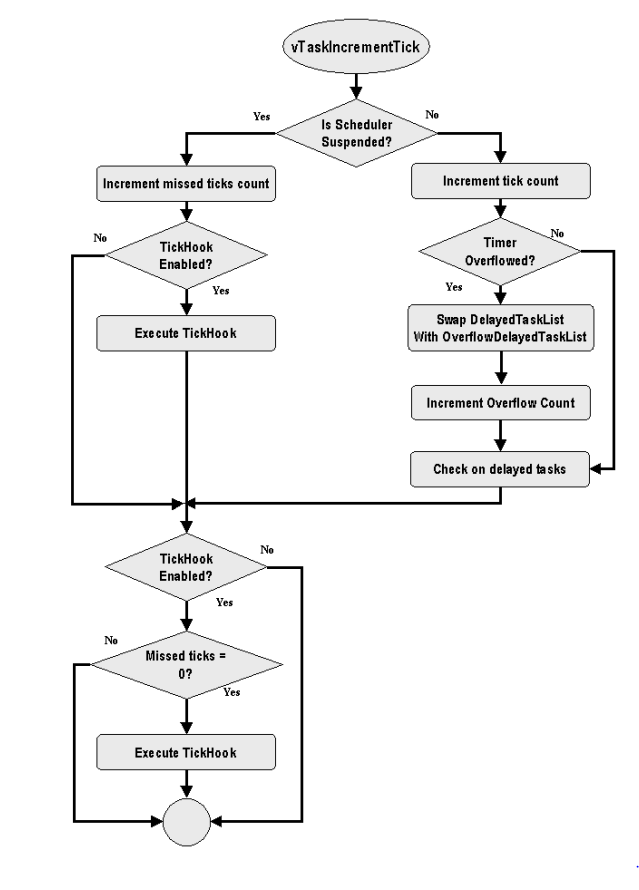
\includegraphics[width=0.8\linewidth]{images/freertos_scheduler_increment.png}
      \caption{vTaskIncrementTick algorithm\citep[p~23]{freertos_inner_workings}}
      \label{fig:freertos_scheduler_increment}
    
\end{figure}

More about the scheduler can be found in \citep{freertos_inner_workings}.

\section{Inner workings of the timers}

Similarly to tasks FreeRTOS timer have a control block. Timer's control block contains timers period, name, does it auto reload and list item. List item is used when a timer is put in a list.  Active timers are stored in current timer list in order of expiry time, first element is the one that will expire first.

When timers are included from the configuration, scheduler on start up  creates the timer daemon service (its priority is modifiable with configTIMER\textunderscore TASK\textunderscore PRIORITY). Timer daemon has a job of processing the expired timers and receiving the commands. All commands controlling the timers the commands are not sent directly to the requested timer, rather all commands are sent to the queue to be later processed by the timer's daemon.

Timer deamon normally just waits for unblocking of the next timer or a new commands from the queue. When a timer expires daemon is woken up, it processes the timer, checks again for received commands and goes back to waiting. If a new commands has arrived the same is expected, first the commands is processed than the task goes back to waiting.
